\documentclass[14pt,a4paper,report]{report}
\usepackage[a4paper, mag=1000, left=2.5cm, right=1cm, top=2cm, bottom=2cm, headsep=0.7cm, footskip=1cm]{geometry}
\usepackage[utf8]{inputenc}
\usepackage[english,russian]{babel}
\usepackage{indentfirst}
\usepackage[dvipsnames]{xcolor}
\usepackage[colorlinks]{hyperref}
\usepackage{listings} 
\usepackage{fancyhdr}
\usepackage{caption}
\usepackage{graphicx}
\hypersetup{
	colorlinks = true,
	linkcolor  = black
}

\usepackage{titlesec}
\titleformat{\chapter}
{\Large\bfseries} % format
{}                % label
{0pt}             % sep
{\huge}           % before-code


\DeclareCaptionFont{white}{\color{white}} 

% Listing description
\usepackage{listings} 
\DeclareCaptionFormat{listing}{\colorbox{gray}{\parbox{\textwidth}{#1#2#3}}}
\captionsetup[lstlisting]{format=listing,labelfont=white,textfont=white}
\lstset{ 
	% Listing settings
	inputencoding = utf8,			
	extendedchars = \true, 
	keepspaces = true, 			  	 % Поддержка кириллицы и пробелов в комментариях
	language = C,            	 	 % Язык программирования (для подсветки)
	basicstyle = \small\sffamily, 	 % Размер и начертание шрифта для подсветки кода
	numbers = left,               	 % Где поставить нумерацию строк (слева\справа)
	numberstyle = \tiny,          	 % Размер шрифта для номеров строк
	stepnumber = 1,               	 % Размер шага между двумя номерами строк
	numbersep = 5pt,              	 % Как далеко отстоят номера строк от подсвечиваемого кода
	backgroundcolor = \color{white}, % Цвет фона подсветки - используем \usepackage{color}
	showspaces = false,           	 % Показывать или нет пробелы специальными отступами
	showstringspaces = false,    	 % Показывать или нет пробелы в строках
	showtabs = false,           	 % Показывать или нет табуляцию в строках
	frame = single,              	 % Рисовать рамку вокруг кода
	tabsize = 2,                  	 % Размер табуляции по умолчанию равен 2 пробелам
	captionpos = t,             	 % Позиция заголовка вверху [t] или внизу [b] 
	breaklines = true,           	 % Автоматически переносить строки (да\нет)
	breakatwhitespace = false,   	 % Переносить строки только если есть пробел
	escapeinside = {\%*}{*)}      	 % Если нужно добавить комментарии в коде
}

\begin{document}

\def\contentsname{Содержание}

% Titlepage
\begin{titlepage}
	\begin{center}
		\textsc{Санкт-Петербургский Политехнический 
			Университет Петра Великого\\[5mm]
			Кафедра компьютерных систем и программных технологий}
		
		\vfill
		
		\textbf{Отчёт по лабораторной работе №2\\[3mm]
			Курс: «Операционные системы»\\[6mm]
			Тема: «Файловые системы»\\[35mm]
		}
	\end{center}
	
	\hfill
	\begin{minipage}{.5\textwidth}
		Выполнил студент:\\[2mm] 
		Бояркин Никита Сергеевич\\
		Группа: 43501/3\\[5mm]
		
		Проверил:\\[2mm] 
		Душутина Елена Владимировна
	\end{minipage}
	\vfill
	\begin{center}
		Санкт-Петербург\\ \the\year\ г.
	\end{center}
\end{titlepage}

% Contents
\tableofcontents
\clearpage

\chapter{Лабораторная работа №2}

\section{Цель работы}

\begin{itemize}
	\item Изучение принципов написания скриптов.
	\item Ознакомление с файловой системой.
	\item Изучение информации о правах владения и доступа к файлу.
	\item Изучение информации о точках монтирования.
\end{itemize}

\section{Программа работы}

\begin{enumerate}
	\item Ознакомиться с типами файлов исследуемой ФС.
	\item Получить все жесткие ссылки на заданный файл.
	\item Проанализировать все возможные способы формирования символьных ссылок.
	\item Получить все символьные ссылки на заданный в качестве входного параметра файл, не используя file.
	\item Изучить утилиту find, используя ее ключи получить расширенную информацию о всех типах файлов.
	\item Проанализировать содержимое заголовка файла, а также файла-каталога. 
	\item Определить максимальное количество записей в каталоге.
	\item Ознакомиться с содержимым /etc/passwd, /etc/shadow, с утилитой /usr/bin/passwd.
	\item Исследовать права владения и доступа, а также их сочетаемость. 
	\begin{enumerate}
		\item Привести примеры применения утилит chmod, chown к специально созданному для этих целей отдельному каталогу с файлами. 
		\item Расширить права исполнения экспериментального файла с помощью флага SUID. 
		\item Экспериментально установить, как формируются итоговые права на использование файла, если права пользователя и группы, в которую он входит, различны.
		\item Сопоставить возможности исполнения наиболее часто используемых операций, варьируя правами доступа к файлу и каталогу.
	\end{enumerate}
	\item Разработать «программу-шлюз» для доступа к файлу другого пользователя при отсутствии прав на чтение информации из этого файла. 
	\item Применяя утилиту df, а также информационные файлы типа fstab, получить информацию о файловых системах, возможных для монтирования. 
	\begin{enumerate}
		\item Привести информацию об исследованных утилитах и информационных файлах с анализом их содержимого и форматов. 
		\item Привести образ диска с точки зрения состава и размещения всех ФС на испытуемом компьютере, а также образ полного дерева ФС, включая присоединенные ФС съемных и несъемных носителей. 
		\item Привести «максимально возможное» дерево ФС, проанализировать, где это указывается
	\end{enumerate}
	\item Проанализировать и пояснить принцип работы утилиты file.  
		\begin{enumerate}
			\item Привести алгоритм её функционирования на основе информационной базы, размещение и полное имя которой указывается в описании утилиты в технической документации ОС.
			\item Утилиту file выполнить с разными ключами. 
			\item  Привести экспериментальную попытку с добавлением в базу собственного типа файла и его дальнейшей идентификацией.
		\end{enumerate}
\end{enumerate}

\section{Характеристики системы}

Некоторая информация об операционной системе и текущем пользователе:

\lstinputlisting{listings/0.my.log}

Информация об операционной системе и текущем пользователе компьютера в лаборатории:

\lstinputlisting{listings/0.lab.log}

На домашнем и лабораторном компьютерах установлены реальные системы.

\section{Ход работы}

\subsection{Фильтрация по одному примеру каждого типа файла}

\subsubsection{Решение в командной строке}

Разработаем команду, которая выведет по одному примеру каждого типа файла из корневого каталога:

\lstinputlisting{listings/1.log}

Рассмотрим команду подробно:

\begin{itemize}
	\item \emph{ls / -l -R} - устанавливаем рекурсивный поиск по корневому каталогу с выводом полной информации.
	\item \emph{2>/dev/null} - перенаправление потока ошибок в никуда.
	\item \emph{awk} - скрипт, который добавляет полный путь в название файла.
	\item \emph{if (\$0\textasciitilde/\textasciicircum\textbackslash//) path=substr(\$0, 0, length(\$0)); } - если строка начинается с / (каталог), то сохраняем текущий путь в переменную.
	\item \emph{else \{ if(\$0\textasciitilde/\textasciicircum1/) \$(NF-2)=path"/"\$(NF-2);} - иначе, если это символьная ссылка (начинается с l), то изменяем путь в столбце (NF-2).
	\item \emph{else \{\$NF=path"/"\$NF\} print \$0\} \} } - иначе заменяем путь в последнем столбце (NF).
	\item \emph{grep -v \textasciicircum/} - избавляемся от вывода каталогов.
	\item \emph{sort -k1.1,1.1} - сортировка по первому символу.
	\item \emph{uniq -w1} - уникальность по первому символу.
\end{itemize}

\clearpage

В результате работы команды были получены типы файлов с префиксами \emph{-, b, c, d, l, p, s}. Рассмотрим каждый префикс подробнее:

\begin{itemize}
	\item \emph{-} файл, обеспечивает хранение символьных и двоичных данных.
	\item \emph{b} - блочное устройство, обеспечивает обращение к аппаратному обеспечению компьютера. Пример блочного устройства - жесткий диск.
	\item \emph{c} - символьное устройство, обеспечивает обращение к аппаратному обеспечению компьютера. Пример символьного устройства - терминал.
	\item \emph{d} - каталог, обеспечивает организацию доступа к файлам.
	\item \emph{l} - символьная ссылка, обеспечивает предоставление доступа к файлам, расположенным на любых носителях.
	\item \emph{p} - канал (FIFO), обеспечивает организацию взаимодействия процессов в операционной системе.
	\item \emph{s} - сокет, обеспечивает организацию взаимодействия процессов в операционной системе.
\end{itemize}

Скрипт был запущен на компьютере в лаборатории, ошибок в работе скрипта не возникало.

\subsubsection{Решение в виде bash скрипта}

Решение аналогично предыдущему пункту, однако оформлено в виде \emph{bash} скрипта. Отличие заключается в получении имени файла из аргументов командной строки и запись решения в этот файл:

\lstinputlisting{listings/1.sh}

Запуск скрипта на исполнение происходит следующим образом:

\begin{verbatim}
nikita@nikita-pc:~/temp1$ sudo sh 1.sh filename
\end{verbatim}

В папке со скриптом создался файл \emph{filename}, в котором находится результат работы скрипта, аналогичный предыдущему пункту. 

Скрипт был запущен на компьютере в лаборатории, ошибок в работе скрипта не возникало.

\subsection{Получение всех жестких ссылок на файл}

С помощью использования индексного дескриптора найдем все ссылки на указанный файл:

\lstinputlisting{listings/2.sh}

Результаты работы скрипта:

\lstinputlisting{listings/2.log}

Проверим работу скрипта на лабораторном компьютере:

\lstinputlisting{listings/2.lab.log}

Скрипт успешно нашел все ссылки жесткие ссылки на файл.

\subsection{Анализ всех способов формирования ссылок}

Рассмотрим действия команд \emph{link, ln, ln -s, cp}. С помощью команды \emph{ls -l} выясним какого рода объекты они порождают:

\lstinputlisting{listings/3.log}

Сделаем вывод о назначении команд \emph{link, ln, ln -s, cp}: 

\begin{itemize}
	\item \emph{link} - позволяет создавать только жесткие ссылки.
	\item \emph{ln} - без ключей создает жесткую ссылку на файл.
	\item \emph{ln -s} - с ключем \emph{-s} создает символьную ссылку на файл.
	\item \emph{cp} - создает новый файл.
\end{itemize}

\subsubsection{Вывод всех полноименных символьных ссылок на файл}

Напишем скрипт подсчитывающий все полноименные символьные ссылки на указанный файл:

\lstinputlisting{listings/3.sh}

Алгоритм работы скрипта, который добавляет полный путь файла и алгоритм перенаправления потока ошибок идентичен скрипту фильтрации каждого типа файла из начала работы.

Результат работы скрипта:

\lstinputlisting{listings/3.r.log}

Проверим работу скрипта на лабораторном компьютере:

\lstinputlisting{listings/3.lab.log}

Скрипт успешно нашел все ссылки символьные ссылки на заданный файл.

\subsection{Вывод всех символьных ссылок на файл}

Напишем скрипт подсчитывающий все символьные ссылки на указанный файл:

\lstinputlisting{listings/4.sh}

Результат работы скрипта:

\lstinputlisting{listings/4.log}

Скрипт был запущен на компьютере в лаборатории, ошибок в работе скрипта не возникало.

\subsection{Утилита find}

\emph{find} - утилита для поиска файлов по имени и другим свойствам в UNIX-подобных ОС. Может проводить поиск в одном или нескольких каталогах, с использованием критериев, заданных пользователем. По умолчанию возвращает все файлы в рабочей директории. также \emph{find} позволяет применять действия ко всем найденным файлам.

Рассмотрим возможности команды \emph{find} с несколькими ключами:

\lstinputlisting{listings/5.log}

Рассмотрим результат исследования команды с несколькими ключами подробнее:

\begin{itemize}
	\item \emph{find -type} - осуществляет поиск по типу файла.
	\item \emph{find -name} - осуществляет поиск файлов по имени, в основном используется для поиска по маске.
	\item \emph{find -size} - осуществляет поиск файлов по размеру. Можно устанавливать нижнюю границу размера файла, верхнюю или обе вместе.
	\item \emph{find -exec} - позволяет создавать вложенные команды. Аргумент "\{\}" заменяется на имя рассматриваемого файла, каждый раз, когда он встречается среди аргументов команды. Все символы за флагом \emph{-exec} считаются ее аргументами до символа ";".
\end{itemize}

\subsection{Утилиты od и hexdump}

Рассмотрим команду \emph{od} с флагами \emph{-c, -bc} на примере тестового файла:

\lstinputlisting{listings/6.o.log}

Рассмотрим используемые команды:

\begin{itemize}
	\item \emph{od} - выводит содержимое файла в восьмеричном формате.
	\item \emph{od -c} - флаг \emph{-c} печатает те символы, которые может напечатать.
	\item \emph{od -bc} - флаг \emph{-b} разбивает результат на октавы.
\end{itemize}

Рассмотрим команду \emph{hexdump}. Она похожа на команду \emph{od}, однако имеет больше возможностей для отображения файла:

\lstinputlisting{listings/6.h.log}

Рассмотрим используемые флаги и форматы:

\begin{itemize}
	\item \emph{-C} - выводит содержимое файла в шестнадцатиричном формате и выводит ASCII символы.
	\item \emph{-e} - позволяет выводить в настраиваемом формате.
	\item \emph{"2\_ad | "} - вывод двух символов смещения в десятичном формате с разделителем "|". 
	\item \emph{2 "\%\_c"} - далее двух символов из файла. 
	\item \emph{$"$| \textbackslash n"} - далее разделитель и символ перевода строки. 
\end{itemize}

\subsection{Определение максимального количества записей в каталоге}

В первой лабораторной работе я выяснил, что размер каталога при создании равен 4096 байт. Это обусловлено типом файловой системы (в данном случае \emph{ext4}). Однако размер каталога можно увеличить, наполняя его файлами или другими каталогами. С помощью скрипта создадим промежуточную папку и будем увеличивать ее размер, наполняя другими каталогами. Если размер папки изменился, то выходим из цикла:

\lstinputlisting{listings/7.sh}

Результат подсчета количества вложенных каталогов для изменения размера папки:

\lstinputlisting{listings/7.log}

Для изменения размера папки с 4096 байт на новое значение понадобилось 340 вложенных каталогов.

Для файловой системы \emph{ext4} максимальное количество каталогов, которое может быть помещено в папку равно $2^{32}-1$.

Скрипт был запущен на компьютере в лаборатории, ошибок в работе скрипта не возникало.

\subsection{Содержимое /etc/passwd, /etc/shadow, утилита passwd}

Рассмотрим содержимое файла \emph{/etc/passwd}:

\lstinputlisting{listings/8.ep.log}

Этот файл содержит строки следующего вида:

\begin{verbatim}
login:passwd:UID:GID:GECOS:home:shell
\end{verbatim}

\begin{itemize}
	\item \emph{login} - имя пользователя.
	\item \emph{passwd} - хэш пароля.
	\item \emph{UID} - уникальный идентификатор пользователя.
	\item \emph{GID} - уникальный идентификатор группы.
	\item \emph{GECOS} - расширенное описание пользователя.
	\item \emph{home} - домашний каталог
	\item \emph{shell} - интерпретатор командной строки.
\end{itemize}

Рассмотрим содержимое файла \emph{/etc/shadow}:

\lstinputlisting{listings/8.es.log}

Этот файл содержит зашифрованную информацию о паролях для всех аккаунтов.

Рассмотрим поля каждой строки файла:

\begin{itemize}
	\item Имя пользователя.
	\item Хэш пароля.
	\item Дата последнего изменения пароля.
	\item Дни до возможности смены пароля.
	\item Дни до устаревания пароля.
	\item За сколько дней до того, как пароль устаревает начинает напоминать о необходимости смены пароля.
	\item Через сколько дней после того, как пароль устареет, заблокировать учетную запись пользователя.
	\item Дата, при достижении которой учетная запись блокируется.
	\item Зарезервированное поле.
\end{itemize}

Утилита \emph{passwd} позволяет изменить пароль текущего пользователя, информацию об учетной записи и срок действия пароля. Суперпользователь может работать с паролями всех пользователей, а остальные пользователи - только со своими паролями. Рассмотрим утилиту \emph{passwd}:

\lstinputlisting{listings/8.p.log}

Некоторые ключи утилиты \emph{passwd}:

\begin{itemize}
	\item \emph{-d} - удалить пароль, учетная запись станет беспарольной.
	\item \emph{-e} - сделать пароль устаревшим.
	\item \emph{-l} - заблокировать пароль пользователя.
	\item \emph{-S} - показать состояние учетной записи.
	\item \emph{-u} - разблокировать пароль пользователя.
\end{itemize}

\subsection{Исследование прав владения и доступа}

\subsubsection{Утилиты chmod, chown}

Исследуем утилиты \emph{chmod} и \emph{chown}:

\lstinputlisting{listings/9.1.log}

Утилита \emph{chmod} предназначена для изменения прав доступа к файлам и директориям. При применении данной команды к каталогу, права вложенных файлов и папок не изменятся. Для изменения прав доступа всех вложенных файлов и папок используется флаг \emph{-R}. 

Утилита \emph{chmod} позволяет задавать права доступа несколькими способами. Рассмотрим эти способы на примере задания прав \emph{rwx---rwx}:

\begin{verbatim}
sudo chmod u=rwx,g=,o=rwx filename
sudo chmod u+rwx,g-rwx,o+rwx filename
sudo chmod 707 filename
\end{verbatim}

Для наглядности в примере была использована символьная форма, однако быстрее и удобнее использовать числовую форму задания прав.

Утилита \emph{chown} предназначена для изменения владельца и/или группы для указанного файла. Владелец и группа задаются через разделитель ":", например \emph{root:root}.

\subsubsection{Расширение прав флагом SUID}

Помимо флага разрешения исполнения \emph{x} существует флаг расширения прав SUID (символ s или S). Этот флаг необходим для запуска пользователем файла, который ему не принадлежит. Флаг S в верхнем регистре используется, если нет прав на выполнение. Попробуем задать расширенные права:

\lstinputlisting{listings/9.2.log}

Также были рассмотрены права утилиты \emph{passwd}. Она также использует флаг расширения прав SUID, для использования несколькими пользователями.

\subsubsection{Формирование итоговых прав, если права пользователя и группы различны}

Сбросим пользовательские права доступа и предоставим все права группе и остальным:

\lstinputlisting{listings/9.3.log}

Несмотря на то, что пользователь принадлежит группе, отсутствие у него прав не позволяет получить доступ к файлу. Это означает, что приоритет пользовательских прав выше прав группы.

\subsubsection{Использование команд записи, чтения и удаления, в зависимости от прав}

Исследуем действие команд записи и чтения файла при различных правах доступа к нему:

\lstinputlisting{listings/9.4.log}

В результате эксперимента было выявлено, что команду \emph{ls -l file} можно использовать к файлу с любыми правами доступа, команду \emph{echo "some" $>$ file} можно использовать только при наличии прав на запись, команду  \emph{cat file} можно использовать только при наличии прав на чтение, команда \emph{rm file} выдаст предупреждение.

\subsection{Разработка программы-шлюза для доступа к файлу другого пользователя}

Разработаем программу-шлюз, которая читает содержимое файла и выводит его в поток вывода:

\lstinputlisting{listings/10.cpp}

Скомпилируем программу на C++ командой:

\begin{verbatim}
g++ -std=c++11 -static-libgcc -static-libstdc++ -o 10.cpp 10.exe
\end{verbatim}

Результат работы программы, запущенной от владельца должен быть аналогичен команде \emph{cat}, убедимся в этом:

\lstinputlisting{listings/10.a.log}

Создадим нового пользователя и от его имени попробуем запустить программу с теми же правами доступа:

\lstinputlisting{listings/10.n.log}

Добавим флаг SUID для программы-шлюза и повторим эксперимент:

\lstinputlisting{listings/10.v.log}

Эксперимент с несколькими пользователями был проведен на компьютере в лаборатории. Результаты эксперимента совпали с ожидаемыми.

\subsection{Получение информации о файловых системах, точках монтирования}

\subsubsection{Утилиты и информационные файлы}

Исследуем утилиту \emph{df} с различными флагами. Утилита \emph{df} предоставляет информацию о состоянии жесткого диска и точках монтирования:

\lstinputlisting{listings/11.d.log}

Утилита \emph{df} выдала 8 точек монтирования, рассмотрим их подробнее:

\begin{itemize}
	\item \emph{udev} - менеджер устройств ядра Linux. Имеет тип \emph{devtmpfs}.
	\item \emph{tmpfs} - одна из разновидностей ФС, отличающаяся быстрой скоростью работы и надежностью. Располагается в оперативной памяти. Имеет тип \emph{tmpfs}.
	\item \emph{/dev/sda1} - основной раздел, отформатированный под Linux. Имеет тип \emph{ext4}.
	\item \emph{/dev/sdb1} - подключенная флешка. Имеет тип \emph{vfat}.
\end{itemize}

Рассмотрим флаги подробнее:

\begin{itemize}
	\item \emph{df -h} - вывод памяти в читабельном формате (килобайты, мегабайты и др.).
	\item \emph{df -i} - вывод памяти в блоках.
	\item \emph{df -T} - вывод информации о типе файловой системы.
\end{itemize}

Рассмотрим ФС с точки зрения физических устройств:

\lstinputlisting{listings/11.ls.log}

В выводе \emph{lsblk} два диска: sda - основной жесткий диск, sdb - флеш накопитель. Основной жесткий диск разделен на три раздела: sda1 - корневой раздел системы в формате \emph{ext4}, sda5 - раздел для виртуальной памяти, sda2 - расширенный раздел, включающий в себя sda5.

Флеш накопитель имеет тип файловой системы \emph{vfat}, который характерен для портативных носителей небольшого объема, и один раздел.

Рассмотрим файл \emph{/etc/fstab}, который содержит информацию о различных файловых системах и устройствах хранения информации:

\lstinputlisting{listings/11.fst.log}

Каждая строка файла \emph{/etc/fstab} имеет структуру:

\begin{verbatim}
<filesystem> <mount point> <type> <options> <dumb> <pass> 
\end{verbatim}

\begin{itemize}
	\item \emph{filesystem} - физическое место размещения файловой системы, по которому определяется конкретный раздел или устройство хранения для монтирования.
	\item \emph{mount point} - точка монтирования, куда монтируется корень файловой системы.
	\item \emph{type} - тип файловой системы. Список всех доступных для монтирования файловых систем определен в файле \emph{/proc/filesystems}.
	\item \emph{options} - параметры монтирования файловой системы.
	\item \emph{dump} - используется утилитой \emph{dump} для определения, нужно ли создать резервную копию данных в файловой системе. Если указана единица, то \emph{dump} создаст резервную копию.
	\item \emph{pass} - используется утилитой \emph{fsck} для определения нужно ли проверять целостность ФС. Значение 1 указывается только для корневой файловой системы. Для остальных ФС следует указывать 2, которое имеет менее высокий приоритет. Если указано 0, то ФС не будет проверяться \emph{fsck}.
\end{itemize}

В файле \emph{/etc/mtab} прописаны устройства, смонтированные в систему в настоящий момент. При монтировании новой ФС в файл будет добавлена соответствующая запись. Формат файла аналогичен формату файла \emph{/etc/fstab}, за исключением того, что в \emph{/etc/mtab} указывается не физический адрес, а путь.

Рассмотрим файл \emph{/etc/mtab}:

\lstinputlisting{listings/11.mt.log}

Список всех доступных для монтирования файловых систем определен в файле \emph{/proc/filesystems}. Рассмотрим его содержимое:

\lstinputlisting{listings/11.fs.log}

Пометка \emph{nodev} говорит о том, что это виртуальная файловая система.

\subsubsection{Максимально возможное дерево файловой системы}

На диске может быть создано не более четырех разделов, это обусловлено тем, что под таблицу разделов в \emph{MBR} выделено 64 байта, а каждая запись занимает 16 байт. Однако это ограничение легко обойти, создав один \emph{Extended} раздел, вместо одного из физических разделов. После этого можно добавить несколько логических разделов. Для примера, создадим несколько разделов, с помощью утилиты \emph{fdisk}:

\lstinputlisting{listings/11.f.log}

Смонтируем в корневую файловую систему четыре файловых системы с флеш накопителя. Построим дерево файловых систем и проверим результат монтирования в файле \emph{/etc/mtab}:

\lstinputlisting{listings/11.m.log}

Теперь при подключении и отключении флеш накопителя будет происходить автоматическое монтирование и размонтирование всех четырех файловых систем.

После монтирования в проводнике операционной системы \emph{Ubuntu} появились все четыре смонтированных файловых системы:

\begin{figure}[h!]
	\centering
	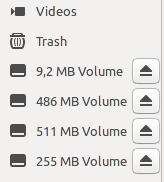
\includegraphics[scale = 0.85]{images/11.png}
	
	\caption{}
	\label{image:1}
\end{figure}

\subsection{Получение информации о файле}

\subsubsection{Магические числа, утилита file}

\emph{file} - специальная утилита, выполняющая ряд проверок для указанного файла, пытаясь его классифицировать. В первую очередь происходит тест на файловую систему, после этого тест на магические числа и языковые тесты.

Тестирование на магические числа выполняется, исходя из информации в файлах \emph{/usr/share/misc/magic}, \emph{/etc/magic} и \emph{/usr/lib/magic}.

Рассмотрим заголовок программы-шлюза \emph{10.exe}, найдем его в одном из вышеуказанных файлов и попробуем классифицировать файл утилитой \emph{file}:

\lstinputlisting{listings/12.1.log}

Заголовок файла \emph{10.exe} содержит в заголовке символы "ELF". Эти символы были найдены в файле \emph{/usr/share/misc/magic}, на основании чего утилита \emph{file} смогла определить тип исследуемого файла.

\subsubsection{Утилита file, примененная к разным типам файлов}

Приведем примеры вывода утилиты \emph{file} при применении на различные типы файлов:

\lstinputlisting{listings/12.2.log}

Утилита \emph{file} определила пустой файл, файл, наполненный исключительно ASCII символами, файл исходного кода \emph{C++} и bash скрипт, содержащий не только ASCII символы.

\subsubsection{Создание собственного типа файлов}

Создадим собственный тип файла. Для этого добавим в \emph{etc/magic} следующую строку:

\begin{verbatim}
0 string MAGIC_HEADER MyType
\end{verbatim}

Теперь любой файл, который с нулевого бита содержит строку \emph{MAGIC\_HEADER} будет иметь тип \emph{MyType}. Проверим это:

\lstinputlisting{listings/12.3.log}

\section{Вывод}

В данной работе была изучена структура файловой системы ОС Linux. В ней существует несколько типов файлов: обычные, директории, ссылки, сокеты, очереди, блок-ориентированные файлы, байт-ориентированные файлы.У одного файла может быть несколько путей, т.е. несколько файлов в структуре каталогов Linux могут быть физически одним файлом на диске. Это достигается тем, что в файловой системе каждый файл идентифицируется уникальным номером, называемым индексным дескриптором. Каждый файл имеет свой индексный дескриптор, идентифицируемый по уникальному номеру, в файловой системе, в которой располагается сам файл.

Также были изучены и экспериментально проверены следующие утилиты: ls, file, od, hexdump, df, fdisk и др.

Были исследованы способы изменения прав доступа и владельца файла. Были проведены эксперименты с флагом SUID.

\clearpage

\section{Список литературы}

\begin{itemize}
	\item Мануал awk [Электронный ресурс]. — URL: \href{https://www.opennet.ru/man.shtml?topic=awk}{https://www.opennet.ru/man.shtml?topic=awk} (дата обращения 20.10.2016).
	\item Мануал cp [Электронный ресурс]. — URL: \href{https://www.opennet.ru/man.shtml?topic=cp}{https://www.opennet.ru/man.shtml?topic=cp} (дата обращения 20.10.2016).
	\item Мануал file [Электронный ресурс]. — URL: \href{https://www.opennet.ru/man.shtml?topic=file}{https://www.opennet.ru/man.shtml?topic=file} (дата обращения 20.10.2016).
	\item Мануал find [Электронный ресурс]. — URL: \href{https://www.opennet.ru/man.shtml?topic=find}{https://www.opennet.ru/man.shtml?topic=find} (дата обращения 20.10.2016).
	\item Мануал fstab [Электронный ресурс]. — URL: \href{https://www.opennet.ru/man.shtml?topic=fstab1}{https://www.opennet.ru/man.shtml?topic=fstab} (дата обращения 20.10.2016).
	\item Мануал hexdump [Электронный ресурс]. — URL: \href{https://www.opennet.ru/man.shtml?topic=hexdump}{https://www.opennet.ru/man.shtml?topic=hexdump} (дата обращения 20.10.2016).
	\item Мануал link [Электронный ресурс]. — URL: \href{https://www.opennet.ru/man.shtml?topic=link}{https://www.opennet.ru/man.shtml?topic=link} (дата обращения 20.10.2016).
	\item Мануал ln [Электронный ресурс]. — URL: \href{https://www.opennet.ru/man.shtml?topic=ln}{https://www.opennet.ru/man.shtml?topic=ln} (дата обращения 20.10.2016).
	\item Мануал od [Электронный ресурс]. — URL: \href{https://www.opennet.ru/man.shtml?topic=od}{https://www.opennet.ru/man.shtml?topic=od} (дата обращения 20.10.2016).
	\item Мануал passwd [Электронный ресурс]. — URL: \href{https://www.opennet.ru/man.shtml?topic=passwd}{https://www.opennet.ru/man.shtml?topic=passwd} (дата обращения 20.10.2016).
	\item Типы файлов в Linux [Электронный ресурс]. — URL: \href{http://younglinux.info/filestype} {http://younglinux.info/filestype} (дата обращения 20.10.2016).
	\item Файл /etc/passwd [Электронный ресурс]. — URL: \href{https://ru.wikipedia.org/wiki//etc/passwd} {https://ru.wikipedia.org/wiki//etc/passwd} (дата обращения 20.10.2016).
\end{itemize}

\end{document}